\documentclass[1p]{elsarticle_modified}
%\bibliographystyle{elsarticle-num}

%\usepackage[colorlinks]{hyperref}
%\usepackage{abbrmath_seonhwa} %\Abb, \Ascr, \Acal ,\Abf, \Afrak
\usepackage{amsfonts}
\usepackage{amssymb}
\usepackage{amsmath}
\usepackage{amsthm}
\usepackage{scalefnt}
\usepackage{amsbsy}
\usepackage{kotex}
\usepackage{caption}
\usepackage{subfig}
\usepackage{color}
\usepackage{graphicx}
\usepackage{xcolor} %% white, black, red, green, blue, cyan, magenta, yellow
\usepackage{float}
\usepackage{setspace}
\usepackage{hyperref}

\usepackage{tikz}
\usetikzlibrary{arrows}

\usepackage{multirow}
\usepackage{array} % fixed length table
\usepackage{hhline}

%%%%%%%%%%%%%%%%%%%%%
\makeatletter
\renewcommand*\env@matrix[1][\arraystretch]{%
	\edef\arraystretch{#1}%
	\hskip -\arraycolsep
	\let\@ifnextchar\new@ifnextchar
	\array{*\c@MaxMatrixCols c}}
\makeatother %https://tex.stackexchange.com/questions/14071/how-can-i-increase-the-line-spacing-in-a-matrix
%%%%%%%%%%%%%%%

\usepackage[normalem]{ulem}

\newcommand{\msout}[1]{\ifmmode\text{\sout{\ensuremath{#1}}}\else\sout{#1}\fi}
%SOURCE: \msout is \stkout macro in https://tex.stackexchange.com/questions/20609/strikeout-in-math-mode

\newcommand{\cancel}[1]{
	\ifmmode
	{\color{red}\msout{#1}}
	\else
	{\color{red}\sout{#1}}
	\fi
}

\newcommand{\add}[1]{
	{\color{blue}\uwave{#1}}
}

\newcommand{\replace}[2]{
	\ifmmode
	{\color{red}\msout{#1}}{\color{blue}\uwave{#2}}
	\else
	{\color{red}\sout{#1}}{\color{blue}\uwave{#2}}
	\fi
}

\newcommand{\Sol}{\mathcal{S}} %segment
\newcommand{\D}{D} %diagram
\newcommand{\A}{\mathcal{A}} %arc


%%%%%%%%%%%%%%%%%%%%%%%%%%%%%5 test

\def\sl{\operatorname{\textup{SL}}(2,\Cbb)}
\def\psl{\operatorname{\textup{PSL}}(2,\Cbb)}
\def\quan{\mkern 1mu \triangleright \mkern 1mu}

\theoremstyle{definition}
\newtheorem{thm}{Theorem}[section]
\newtheorem{prop}[thm]{Proposition}
\newtheorem{lem}[thm]{Lemma}
\newtheorem{ques}[thm]{Question}
\newtheorem{cor}[thm]{Corollary}
\newtheorem{defn}[thm]{Definition}
\newtheorem{exam}[thm]{Example}
\newtheorem{rmk}[thm]{Remark}
\newtheorem{alg}[thm]{Algorithm}

\newcommand{\I}{\sqrt{-1}}
\begin{document}

%\begin{frontmatter}
%
%\title{Boundary parabolic representations of knots up to 8 crossings}
%
%%% Group authors per affiliation:
%\author{Yunhi Cho} 
%\address{Department of Mathematics, University of Seoul, Seoul, Korea}
%\ead{yhcho@uos.ac.kr}
%
%
%\author{Seonhwa Kim} %\fnref{s_kim}}
%\address{Center for Geometry and Physics, Institute for Basic Science, Pohang, 37673, Korea}
%\ead{ryeona17@ibs.re.kr}
%
%\author{Hyuk Kim}
%\address{Department of Mathematical Sciences, Seoul National University, Seoul 08826, Korea}
%\ead{hyukkim@snu.ac.kr}
%
%\author{Seokbeom Yoon}
%\address{Department of Mathematical Sciences, Seoul National University, Seoul, 08826,  Korea}
%\ead{sbyoon15@snu.ac.kr}
%
%\begin{abstract}
%We find all boundary parabolic representation of knots up to 8 crossings.
%
%\end{abstract}
%\begin{keyword}
%    \MSC[2010] 57M25 
%\end{keyword}
%
%\end{frontmatter}

%\linenumbers
%\tableofcontents
%
\newcommand\colored[1]{\textcolor{white}{\rule[-0.35ex]{0.8em}{1.4ex}}\kern-0.8em\color{red} #1}%
%\newcommand\colored[1]{\textcolor{white}{ #1}\kern-2.17ex	\textcolor{white}{ #1}\kern-1.81ex	\textcolor{white}{ #1}\kern-2.15ex\color{red}#1	}

{\Large $\underline{12a_{0771}~(K12a_{0771})}$}

\setlength{\tabcolsep}{10pt}
\renewcommand{\arraystretch}{1.6}
\vspace{1cm}\begin{tabular}{m{100pt}>{\centering\arraybackslash}m{274pt}}
\multirow{5}{120pt}{
	\centering
	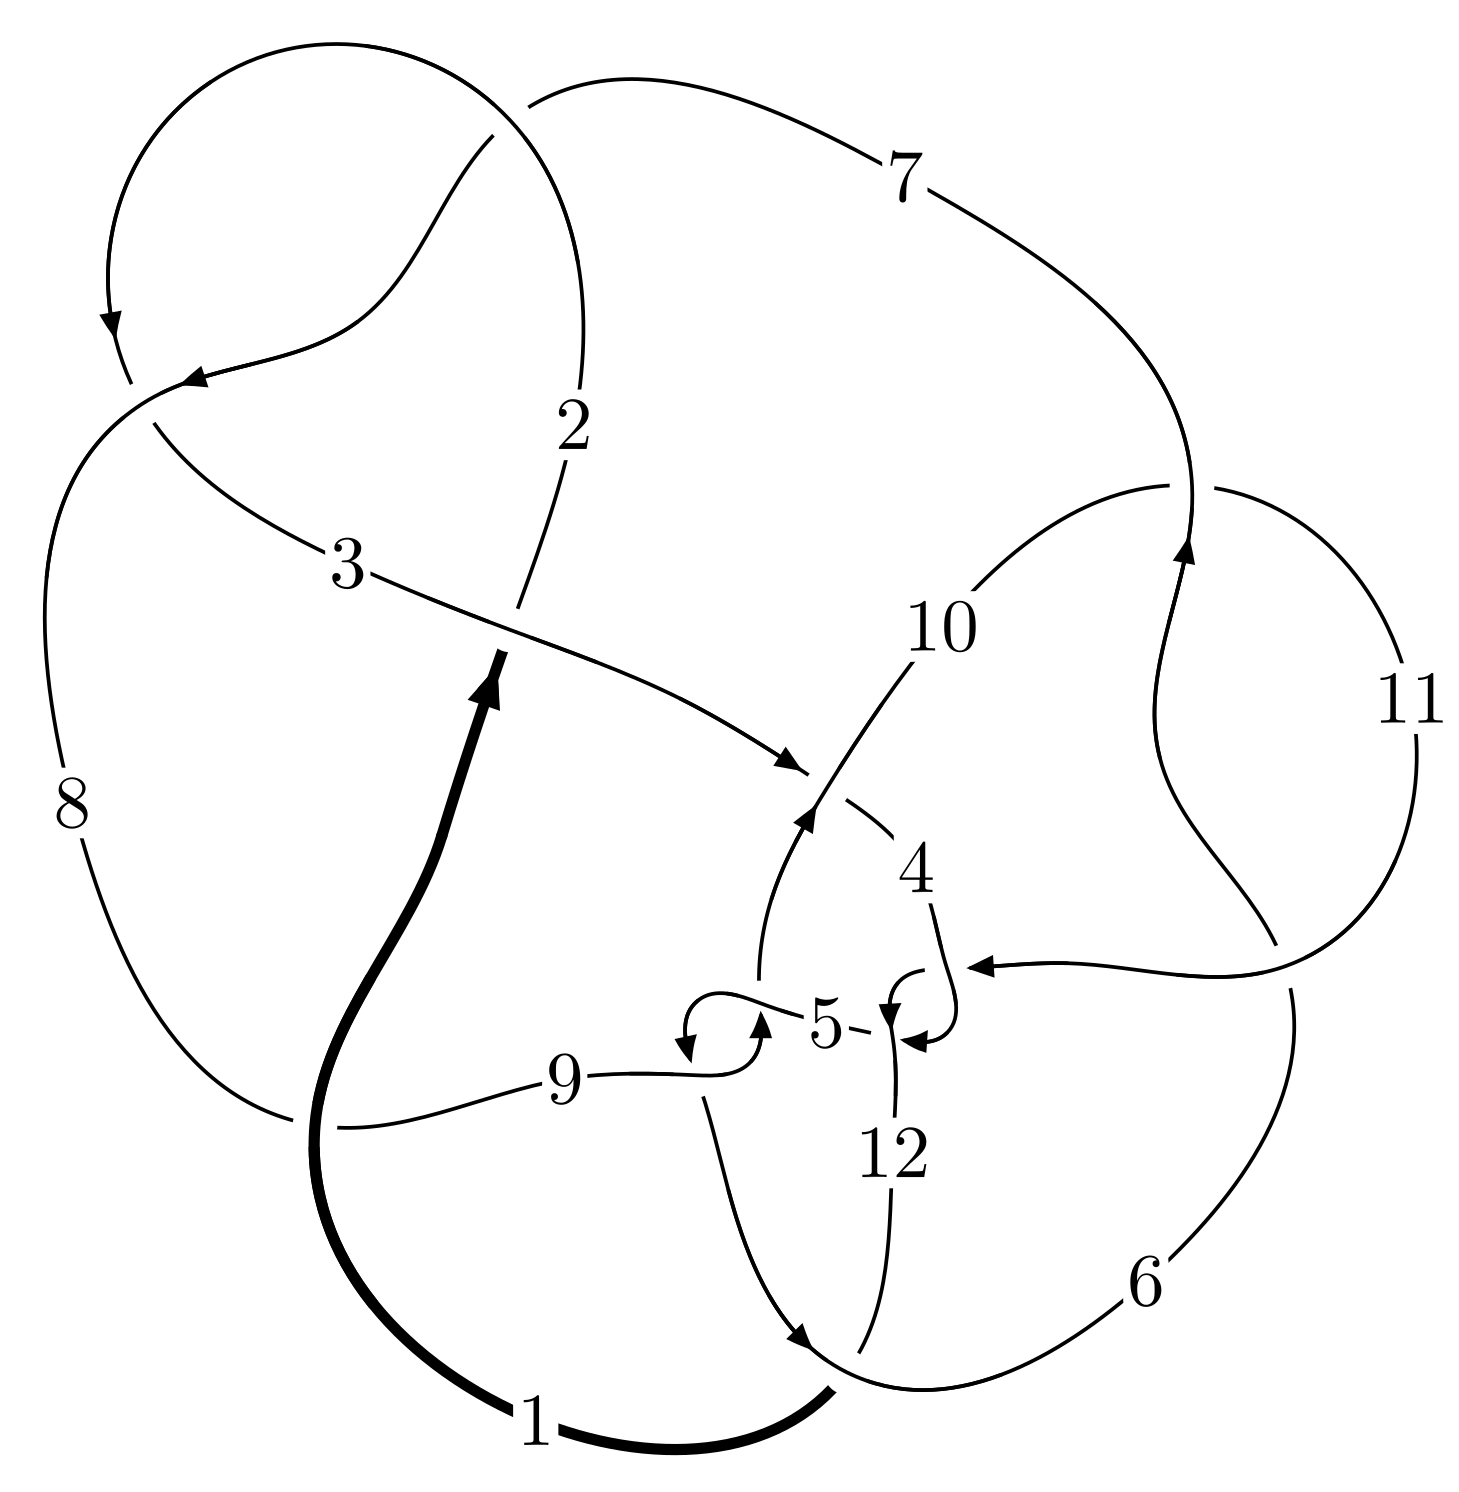
\includegraphics[width=112pt]{../../../GIT/diagram.site/Diagrams/png/1572_12a_0771.png}\\
\ \ \ A knot diagram\footnotemark}&
\allowdisplaybreaks
\textbf{Linearized knot diagam} \\
\cline{2-2}
 &
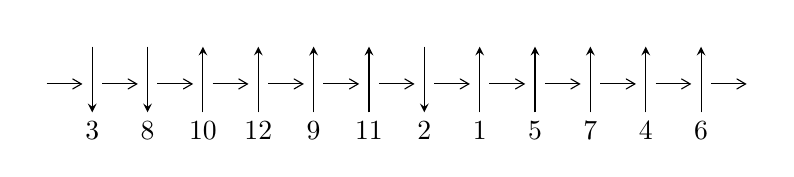
\begin{tikzpicture}[x=20pt, y=17pt]
	% nodes
	\node (C0) at (0, 0) {};
	\node (C1) at (1, 0) {};
	\node (C1U) at (1, +1) {};
	\node (C1D) at (1, -1) {3};

	\node (C2) at (2, 0) {};
	\node (C2U) at (2, +1) {};
	\node (C2D) at (2, -1) {8};

	\node (C3) at (3, 0) {};
	\node (C3U) at (3, +1) {};
	\node (C3D) at (3, -1) {10};

	\node (C4) at (4, 0) {};
	\node (C4U) at (4, +1) {};
	\node (C4D) at (4, -1) {12};

	\node (C5) at (5, 0) {};
	\node (C5U) at (5, +1) {};
	\node (C5D) at (5, -1) {9};

	\node (C6) at (6, 0) {};
	\node (C6U) at (6, +1) {};
	\node (C6D) at (6, -1) {11};

	\node (C7) at (7, 0) {};
	\node (C7U) at (7, +1) {};
	\node (C7D) at (7, -1) {2};

	\node (C8) at (8, 0) {};
	\node (C8U) at (8, +1) {};
	\node (C8D) at (8, -1) {1};

	\node (C9) at (9, 0) {};
	\node (C9U) at (9, +1) {};
	\node (C9D) at (9, -1) {5};

	\node (C10) at (10, 0) {};
	\node (C10U) at (10, +1) {};
	\node (C10D) at (10, -1) {7};

	\node (C11) at (11, 0) {};
	\node (C11U) at (11, +1) {};
	\node (C11D) at (11, -1) {4};

	\node (C12) at (12, 0) {};
	\node (C12U) at (12, +1) {};
	\node (C12D) at (12, -1) {6};
	\node (C13) at (13, 0) {};

	% arrows
	\draw[->,>={angle 60}]
	(C0) edge (C1) (C1) edge (C2) (C2) edge (C3) (C3) edge (C4) (C4) edge (C5) (C5) edge (C6) (C6) edge (C7) (C7) edge (C8) (C8) edge (C9) (C9) edge (C10) (C10) edge (C11) (C11) edge (C12) (C12) edge (C13) ;	\draw[->,>=stealth]
	(C1U) edge (C1D) (C2U) edge (C2D) (C3D) edge (C3U) (C4D) edge (C4U) (C5D) edge (C5U) (C6D) edge (C6U) (C7U) edge (C7D) (C8D) edge (C8U) (C9D) edge (C9U) (C10D) edge (C10U) (C11D) edge (C11U) (C12D) edge (C12U) ;
	\end{tikzpicture} \\
\hhline{~~} \\& 
\textbf{Solving Sequence} \\ \cline{2-2} 
 &
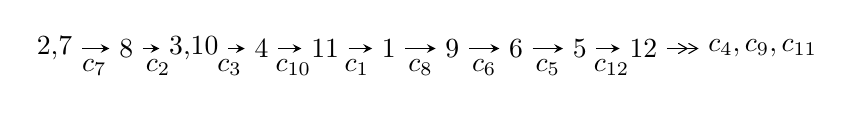
\begin{tikzpicture}[x=23pt, y=7pt]
	% node
	\node (A0) at (-1/8, 0) {2,7};
	\node (A1) at (1, 0) {8};
	\node (A2) at (33/16, 0) {3,10};
	\node (A3) at (25/8, 0) {4};
	\node (A4) at (33/8, 0) {11};
	\node (A5) at (41/8, 0) {1};
	\node (A6) at (49/8, 0) {9};
	\node (A7) at (57/8, 0) {6};
	\node (A8) at (65/8, 0) {5};
	\node (A9) at (73/8, 0) {12};
	\node (C1) at (1/2, -1) {$c_{7}$};
	\node (C2) at (3/2, -1) {$c_{2}$};
	\node (C3) at (21/8, -1) {$c_{3}$};
	\node (C4) at (29/8, -1) {$c_{10}$};
	\node (C5) at (37/8, -1) {$c_{1}$};
	\node (C6) at (45/8, -1) {$c_{8}$};
	\node (C7) at (53/8, -1) {$c_{6}$};
	\node (C8) at (61/8, -1) {$c_{5}$};
	\node (C9) at (69/8, -1) {$c_{12}$};
	\node (A10) at (11, 0) {$c_{4},c_{9},c_{11}$};

	% edge
	\draw[->,>=stealth]	
	(A0) edge (A1) (A1) edge (A2) (A2) edge (A3) (A3) edge (A4) (A4) edge (A5) (A5) edge (A6) (A6) edge (A7) (A7) edge (A8) (A8) edge (A9) ;
	\draw[->>,>={angle 60}]	
	(A9) edge (A10);
\end{tikzpicture} \\ 

\end{tabular} \\

\footnotetext{
The image of knot diagram is generated by the software ``\textbf{Draw programme}" developed by Andrew Bartholomew(\url{http://www.layer8.co.uk/maths/draw/index.htm\#Running-draw}), where we modified some parts for our purpose(\url{https://github.com/CATsTAILs/LinksPainter}).
}\phantom \\ \newline 
\centering \textbf{Ideals for irreducible components\footnotemark of $X_{\text{par}}$} 
 
\begin{align*}
I^u_{1}&=\langle 
8.94153\times10^{27} u^{43}+1.81790\times10^{28} u^{42}+\cdots+2.63209\times10^{28} b-4.42452\times10^{28},\\
\phantom{I^u_{1}}&\phantom{= \langle  }-1.06493\times10^{29} u^{43}-2.17847\times10^{29} u^{42}+\cdots+1.05284\times10^{29} a-5.20010\times10^{29},\\
\phantom{I^u_{1}}&\phantom{= \langle  }u^{44}+3 u^{43}+\cdots+12 u+8\rangle \\
I^u_{2}&=\langle 
-2 u^{35} a+2 u^{35}+\cdots+3 a+2,\;30 u^{35} a-138 u^{35}+\cdots-15 a+144,\;u^{36}- u^{35}+\cdots- u^2+1\rangle \\
I^u_{3}&=\langle 
b-1,\;- u^3+4 u^2+4 a-2,\;u^4-2 u^2+2\rangle \\
\\
I^v_{1}&=\langle 
a,\;b+1,\;2 v+1\rangle \\
\end{align*}
\raggedright * 4 irreducible components of $\dim_{\mathbb{C}}=0$, with total 121 representations.\\
\footnotetext{All coefficients of polynomials are rational numbers. But the coefficients are sometimes approximated in decimal forms when there is not enough margin.}
\newpage
\renewcommand{\arraystretch}{1}
\centering \section*{I. $I^u_{1}= \langle 8.94\times10^{27} u^{43}+1.82\times10^{28} u^{42}+\cdots+2.63\times10^{28} b-4.42\times10^{28},\;-1.06\times10^{29} u^{43}-2.18\times10^{29} u^{42}+\cdots+1.05\times10^{29} a-5.20\times10^{29},\;u^{44}+3 u^{43}+\cdots+12 u+8 \rangle$}
\flushleft \textbf{(i) Arc colorings}\\
\begin{tabular}{m{7pt} m{180pt} m{7pt} m{180pt} }
\flushright $a_{2}=$&$\begin{pmatrix}0\\u\end{pmatrix}$ \\
\flushright $a_{7}=$&$\begin{pmatrix}1\\0\end{pmatrix}$ \\
\flushright $a_{8}=$&$\begin{pmatrix}1\\u^2\end{pmatrix}$ \\
\flushright $a_{3}=$&$\begin{pmatrix}- u\\- u^3+u\end{pmatrix}$ \\
\flushright $a_{10}=$&$\begin{pmatrix}1.01148 u^{43}+2.06914 u^{42}+\cdots+6.75356 u+4.93913\\-0.339712 u^{43}-0.690668 u^{42}+\cdots+0.899245 u+1.68099\end{pmatrix}$ \\
\flushright $a_{4}=$&$\begin{pmatrix}-0.491722 u^{43}-1.08414 u^{42}+\cdots-5.99398 u-7.66894\\0.0371897 u^{43}+0.0225085 u^{42}+\cdots+0.0962924 u+0.243944\end{pmatrix}$ \\
\flushright $a_{11}=$&$\begin{pmatrix}0.671771 u^{43}+1.37847 u^{42}+\cdots+7.65281 u+6.62012\\-0.339712 u^{43}-0.690668 u^{42}+\cdots+0.899245 u+1.68099\end{pmatrix}$ \\
\flushright $a_{1}=$&$\begin{pmatrix}u^3\\u^5- u^3+u\end{pmatrix}$ \\
\flushright $a_{9}=$&$\begin{pmatrix}u^6- u^4+1\\u^8-2 u^6+2 u^4\end{pmatrix}$ \\
\flushright $a_{6}=$&$\begin{pmatrix}-0.410209 u^{43}-0.680680 u^{42}+\cdots-5.44836 u-3.15716\\-0.585333 u^{43}-1.56699 u^{42}+\cdots-0.199466 u-3.32612\end{pmatrix}$ \\
\flushright $a_{5}=$&$\begin{pmatrix}-0.395067 u^{43}-0.647681 u^{42}+\cdots-7.86724 u-6.66270\\-0.214121 u^{43}-0.720629 u^{42}+\cdots+0.874054 u-0.939898\end{pmatrix}$ \\
\flushright $a_{12}=$&$\begin{pmatrix}0.454683 u^{43}+0.926181 u^{42}+\cdots+6.06159 u+5.75581\\-0.205670 u^{43}-0.268381 u^{42}+\cdots-0.997900 u+1.21691\end{pmatrix}$\\&\end{tabular}
\flushleft \textbf{(ii) Obstruction class $= -1$}\\~\\
\flushleft \textbf{(iii) Cusp Shapes $= 0.954565 u^{43}+3.18813 u^{42}+\cdots-26.7876 u+6.14997$}\\~\\
\newpage\renewcommand{\arraystretch}{1}
\flushleft \textbf{(iv) u-Polynomials at the component}\newline \\
\begin{tabular}{m{50pt}|m{274pt}}
Crossings & \hspace{64pt}u-Polynomials at each crossing \\
\hline $$\begin{aligned}c_{1}\end{aligned}$$&$\begin{aligned}
&u^{44}+23 u^{43}+\cdots+272 u+64
\end{aligned}$\\
\hline $$\begin{aligned}c_{2},c_{7}\end{aligned}$$&$\begin{aligned}
&u^{44}+3 u^{43}+\cdots+12 u+8
\end{aligned}$\\
\hline $$\begin{aligned}c_{3},c_{12}\end{aligned}$$&$\begin{aligned}
&128(128 u^{44}+64 u^{43}+\cdots-11 u-1)
\end{aligned}$\\
\hline $$\begin{aligned}c_{4},c_{11}\end{aligned}$$&$\begin{aligned}
&u^{44}-13 u^{42}+\cdots+647 u-416
\end{aligned}$\\
\hline $$\begin{aligned}c_{5},c_{6},c_{9}\\c_{10}\end{aligned}$$&$\begin{aligned}
&u^{44}+u^{43}+\cdots-16 u-5
\end{aligned}$\\
\hline $$\begin{aligned}c_{8}\end{aligned}$$&$\begin{aligned}
&u^{44}+9 u^{43}+\cdots+42988 u+25384
\end{aligned}$\\
\hline
\end{tabular}\\~\\
\newpage\renewcommand{\arraystretch}{1}
\flushleft \textbf{(v) Riley Polynomials at the component}\newline \\
\begin{tabular}{m{50pt}|m{274pt}}
Crossings & \hspace{64pt}Riley Polynomials at each crossing \\
\hline $$\begin{aligned}c_{1}\end{aligned}$$&$\begin{aligned}
&y^{44}-3 y^{43}+\cdots-12544 y+4096
\end{aligned}$\\
\hline $$\begin{aligned}c_{2},c_{7}\end{aligned}$$&$\begin{aligned}
&y^{44}-23 y^{43}+\cdots-272 y+64
\end{aligned}$\\
\hline $$\begin{aligned}c_{3},c_{12}\end{aligned}$$&$\begin{aligned}
&16384(16384 y^{44}+151552 y^{43}+\cdots-55 y+1)
\end{aligned}$\\
\hline $$\begin{aligned}c_{4},c_{11}\end{aligned}$$&$\begin{aligned}
&y^{44}-26 y^{43}+\cdots-5622769 y+173056
\end{aligned}$\\
\hline $$\begin{aligned}c_{5},c_{6},c_{9}\\c_{10}\end{aligned}$$&$\begin{aligned}
&y^{44}+17 y^{43}+\cdots-146 y+25
\end{aligned}$\\
\hline $$\begin{aligned}c_{8}\end{aligned}$$&$\begin{aligned}
&y^{44}+29 y^{43}+\cdots-8202497168 y+644347456
\end{aligned}$\\
\hline
\end{tabular}\\~\\
\newpage\flushleft \textbf{(vi) Complex Volumes and Cusp Shapes}
$$\begin{array}{c|c|c}  
\text{Solutions to }I^u_{1}& \I (\text{vol} + \sqrt{-1}CS) & \text{Cusp shape}\\
 \hline 
\begin{aligned}
u &= -0.884944 + 0.456342 I \\
a &= \phantom{-}1.76169 - 1.31420 I \\
b &= -0.815843 - 0.660997 I\end{aligned}
 & \phantom{-}3.80422 + 3.00198 I & \phantom{-}9.87086 - 5.43823 I \\ \hline\begin{aligned}
u &= -0.884944 - 0.456342 I \\
a &= \phantom{-}1.76169 + 1.31420 I \\
b &= -0.815843 + 0.660997 I\end{aligned}
 & \phantom{-}3.80422 - 3.00198 I & \phantom{-}9.87086 + 5.43823 I \\ \hline\begin{aligned}
u &= -0.670238 + 0.750027 I \\
a &= -0.384753 + 1.126000 I \\
b &= \phantom{-}0.459752 - 1.089540 I\end{aligned}
 & \phantom{-}0.43707 - 6.38433 I & \phantom{-}5.82179 + 5.84528 I \\ \hline\begin{aligned}
u &= -0.670238 - 0.750027 I \\
a &= -0.384753 - 1.126000 I \\
b &= \phantom{-}0.459752 + 1.089540 I\end{aligned}
 & \phantom{-}0.43707 + 6.38433 I & \phantom{-}5.82179 - 5.84528 I \\ \hline\begin{aligned}
u &= -0.601725 + 0.830742 I \\
a &= -0.529924 - 0.448858 I \\
b &= \phantom{-}0.184705 + 0.860484 I\end{aligned}
 & -0.47398 + 2.76828 I & \phantom{-}9.57507 - 9.72155 I \\ \hline\begin{aligned}
u &= -0.601725 - 0.830742 I \\
a &= -0.529924 + 0.448858 I \\
b &= \phantom{-}0.184705 - 0.860484 I\end{aligned}
 & -0.47398 - 2.76828 I & \phantom{-}9.57507 + 9.72155 I \\ \hline\begin{aligned}
u &= \phantom{-}0.186329 + 0.936259 I \\
a &= -0.0808606 - 0.0791166 I \\
b &= -0.073120 + 0.812347 I\end{aligned}
 & \phantom{-}0.435225 - 0.901619 I & \phantom{-}13.9955 + 4.4616 I \\ \hline\begin{aligned}
u &= \phantom{-}0.186329 - 0.936259 I \\
a &= -0.0808606 + 0.0791166 I \\
b &= -0.073120 - 0.812347 I\end{aligned}
 & \phantom{-}0.435225 + 0.901619 I & \phantom{-}13.9955 - 4.4616 I \\ \hline\begin{aligned}
u &= \phantom{-}0.191787 + 0.913705 I \\
a &= \phantom{-}0.872159 + 0.565110 I \\
b &= -0.381936 - 1.276420 I\end{aligned}
 & -7.62519 + 7.08844 I & \phantom{-}1.23316 - 4.93509 I \\ \hline\begin{aligned}
u &= \phantom{-}0.191787 - 0.913705 I \\
a &= \phantom{-}0.872159 - 0.565110 I \\
b &= -0.381936 + 1.276420 I\end{aligned}
 & -7.62519 - 7.08844 I & \phantom{-}1.23316 + 4.93509 I\\
 \hline 
 \end{array}$$\newpage$$\begin{array}{c|c|c}  
\text{Solutions to }I^u_{1}& \I (\text{vol} + \sqrt{-1}CS) & \text{Cusp shape}\\
 \hline 
\begin{aligned}
u &= -0.208206 + 0.873746 I \\
a &= \phantom{-}1.33288 - 0.57705 I \\
b &= -0.57707 + 1.33359 I\end{aligned}
 & -4.2603 - 13.7418 I & \phantom{-}4.56439 + 7.35664 I \\ \hline\begin{aligned}
u &= -0.208206 - 0.873746 I \\
a &= \phantom{-}1.33288 + 0.57705 I \\
b &= -0.57707 - 1.33359 I\end{aligned}
 & -4.2603 + 13.7418 I & \phantom{-}4.56439 - 7.35664 I \\ \hline\begin{aligned}
u &= -1.004180 + 0.480691 I \\
a &= -0.017302 - 0.166511 I \\
b &= -0.289315 + 0.457341 I\end{aligned}
 & -1.31781 + 1.99895 I & \phantom{-}3.76651 + 1.75105 I \\ \hline\begin{aligned}
u &= -1.004180 - 0.480691 I \\
a &= -0.017302 + 0.166511 I \\
b &= -0.289315 - 0.457341 I\end{aligned}
 & -1.31781 - 1.99895 I & \phantom{-}3.76651 - 1.75105 I \\ \hline\begin{aligned}
u &= -0.891355 + 0.676843 I \\
a &= \phantom{-}1.80496 + 0.33828 I \\
b &= -0.524580 - 1.162410 I\end{aligned}
 & -0.21415 + 11.72470 I & \phantom{-}5.05083 - 10.25102 I \\ \hline\begin{aligned}
u &= -0.891355 - 0.676843 I \\
a &= \phantom{-}1.80496 - 0.33828 I \\
b &= -0.524580 + 1.162410 I\end{aligned}
 & -0.21415 - 11.72470 I & \phantom{-}5.05083 + 10.25102 I \\ \hline\begin{aligned}
u &= \phantom{-}1.064910 + 0.482421 I \\
a &= \phantom{-}0.874561 + 0.554909 I \\
b &= -0.432078 + 0.243913 I\end{aligned}
 & -1.04936 - 4.41613 I & \phantom{-}4.34936 + 8.68385 I \\ \hline\begin{aligned}
u &= \phantom{-}1.064910 - 0.482421 I \\
a &= \phantom{-}0.874561 - 0.554909 I \\
b &= -0.432078 - 0.243913 I\end{aligned}
 & -1.04936 + 4.41613 I & \phantom{-}4.34936 - 8.68385 I \\ \hline\begin{aligned}
u &= -0.667044 + 0.444211 I \\
a &= -1.60584 + 0.60607 I \\
b &= \phantom{-}1.020760 - 0.533523 I\end{aligned}
 & \phantom{-}4.44990 + 0.84092 I & \phantom{-}12.07181 - 5.13739 I \\ \hline\begin{aligned}
u &= -0.667044 - 0.444211 I \\
a &= -1.60584 - 0.60607 I \\
b &= \phantom{-}1.020760 + 0.533523 I\end{aligned}
 & \phantom{-}4.44990 - 0.84092 I & \phantom{-}12.07181 + 5.13739 I\\
 \hline 
 \end{array}$$\newpage$$\begin{array}{c|c|c}  
\text{Solutions to }I^u_{1}& \I (\text{vol} + \sqrt{-1}CS) & \text{Cusp shape}\\
 \hline 
\begin{aligned}
u &= \phantom{-}1.136530 + 0.421684 I \\
a &= \phantom{-}0.606451 + 1.237990 I \\
b &= -1.389530 + 0.221504 I\end{aligned}
 & -0.17714 - 2.64557 I & \phantom{-0.000000 }      -6
0. 10   - 1.179168 I \\ \hline\begin{aligned}
u &= \phantom{-}1.136530 - 0.421684 I \\
a &= \phantom{-}0.606451 - 1.237990 I \\
b &= -1.389530 - 0.221504 I\end{aligned}
 & -0.17714 + 2.64557 I & \phantom{-0.000000 -}     -6
0. 10   + 1.179168 I \\ \hline\begin{aligned}
u &= -1.146090 + 0.479405 I \\
a &= \phantom{-}0.239075 - 1.309680 I \\
b &= -1.39337 + 0.38888 I\end{aligned}
 & \phantom{-}0.24666 + 5.31593 I & \phantom{-}2.56328 - 8.44742 I \\ \hline\begin{aligned}
u &= -1.146090 - 0.479405 I \\
a &= \phantom{-}0.239075 + 1.309680 I \\
b &= -1.39337 - 0.38888 I\end{aligned}
 & \phantom{-}0.24666 - 5.31593 I & \phantom{-}2.56328 + 8.44742 I \\ \hline\begin{aligned}
u &= \phantom{-}1.082540 + 0.685582 I \\
a &= \phantom{-}1.011040 + 0.097761 I \\
b &= -0.193861 + 0.889333 I\end{aligned}
 & -2.02935 - 4.79440 I & \phantom{-}7.24675 + 10.74676 I \\ \hline\begin{aligned}
u &= \phantom{-}1.082540 - 0.685582 I \\
a &= \phantom{-}1.011040 - 0.097761 I \\
b &= -0.193861 - 0.889333 I\end{aligned}
 & -2.02935 + 4.79440 I & \phantom{-}7.24675 - 10.74676 I \\ \hline\begin{aligned}
u &= \phantom{-}1.259910 + 0.315100 I \\
a &= \phantom{-}0.091904 + 0.628273 I \\
b &= \phantom{-}0.52009 + 1.36003 I\end{aligned}
 & -8.94132 + 9.79930 I & \phantom{-0.000000 } 0. - 4.91774 I \\ \hline\begin{aligned}
u &= \phantom{-}1.259910 - 0.315100 I \\
a &= \phantom{-}0.091904 - 0.628273 I \\
b &= \phantom{-}0.52009 - 1.36003 I\end{aligned}
 & -8.94132 - 9.79930 I & \phantom{-0.000000 -}0. + 4.91774 I \\ \hline\begin{aligned}
u &= \phantom{-}0.685053\phantom{ +0.000000I} \\
a &= -1.66669\phantom{ +0.000000I} \\
b &= -0.374180\phantom{ +0.000000I}\end{aligned}
 & \phantom{-}2.00566\phantom{ +0.000000I} & \phantom{-}3.54950\phantom{ +0.000000I} \\ \hline\begin{aligned}
u &= -1.201480 + 0.555428 I \\
a &= -2.04851 + 0.88093 I \\
b &= \phantom{-}0.60384 + 1.36202 I\end{aligned}
 & -7.2417 + 18.9627 I & \phantom{-0.000000 } 0. - 10.45856 I\\
 \hline 
 \end{array}$$\newpage$$\begin{array}{c|c|c}  
\text{Solutions to }I^u_{1}& \I (\text{vol} + \sqrt{-1}CS) & \text{Cusp shape}\\
 \hline 
\begin{aligned}
u &= -1.201480 - 0.555428 I \\
a &= -2.04851 - 0.88093 I \\
b &= \phantom{-}0.60384 - 1.36202 I\end{aligned}
 & -7.2417 - 18.9627 I & \phantom{-0.000000 -}0. + 10.45856 I \\ \hline\begin{aligned}
u &= -1.298400 + 0.319915 I \\
a &= \phantom{-}0.224279 - 0.600246 I \\
b &= \phantom{-}0.287147 - 1.310910 I\end{aligned}
 & -12.44790 - 2.88689 I & -3.91928 + 0. I\phantom{ +0.000000I} \\ \hline\begin{aligned}
u &= -1.298400 - 0.319915 I \\
a &= \phantom{-}0.224279 + 0.600246 I \\
b &= \phantom{-}0.287147 + 1.310910 I\end{aligned}
 & -12.44790 + 2.88689 I & -3.91928 + 0. I\phantom{ +0.000000I} \\ \hline\begin{aligned}
u &= \phantom{-}1.330060 + 0.160088 I \\
a &= \phantom{-}0.223696 + 0.671956 I \\
b &= -0.211250 + 1.150130 I\end{aligned}
 & -7.05764 - 5.66751 I & -3.71453 + 8.78354 I \\ \hline\begin{aligned}
u &= \phantom{-}1.330060 - 0.160088 I \\
a &= \phantom{-}0.223696 - 0.671956 I \\
b &= -0.211250 - 1.150130 I\end{aligned}
 & -7.05764 + 5.66751 I & -3.71453 - 8.78354 I \\ \hline\begin{aligned}
u &= \phantom{-}1.219740 + 0.558773 I \\
a &= -1.69862 - 0.67374 I \\
b &= \phantom{-}0.423980 - 1.324410 I\end{aligned}
 & -10.7383 - 12.4231 I & \phantom{-0.000000 -}0. + 7.73932 I \\ \hline\begin{aligned}
u &= \phantom{-}1.219740 - 0.558773 I \\
a &= -1.69862 + 0.67374 I \\
b &= \phantom{-}0.423980 + 1.324410 I\end{aligned}
 & -10.7383 + 12.4231 I & \phantom{-0.000000 } 0. - 7.73932 I \\ \hline\begin{aligned}
u &= -0.126816 + 0.631710 I \\
a &= -1.75809 - 0.34785 I \\
b &= \phantom{-}1.283540 + 0.336498 I\end{aligned}
 & \phantom{-}3.08765 - 1.01915 I & \phantom{-}6.08245 + 6.44104 I \\ \hline\begin{aligned}
u &= -0.126816 - 0.631710 I \\
a &= -1.75809 + 0.34785 I \\
b &= \phantom{-}1.283540 - 0.336498 I\end{aligned}
 & \phantom{-}3.08765 + 1.01915 I & \phantom{-}6.08245 - 6.44104 I \\ \hline\begin{aligned}
u &= \phantom{-}0.643966\phantom{ +0.000000I} \\
a &= -1.64514\phantom{ +0.000000I} \\
b &= \phantom{-}1.21259\phantom{ +0.000000I}\end{aligned}
 & \phantom{-}2.74899\phantom{ +0.000000I} & -5.75340\phantom{ +0.000000I}\\
 \hline 
 \end{array}$$\newpage$$\begin{array}{c|c|c}  
\text{Solutions to }I^u_{1}& \I (\text{vol} + \sqrt{-1}CS) & \text{Cusp shape}\\
 \hline 
\begin{aligned}
u &= \phantom{-}0.378525 + 0.481692 I \\
a &= -1.018580 - 0.068518 I \\
b &= \phantom{-}0.389924 + 0.119878 I\end{aligned}
 & \phantom{-}0.917264 + 0.353906 I & \phantom{-}10.71011 - 2.76595 I \\ \hline\begin{aligned}
u &= \phantom{-}0.378525 - 0.481692 I \\
a &= -1.018580 + 0.068518 I \\
b &= \phantom{-}0.389924 - 0.119878 I\end{aligned}
 & \phantom{-}0.917264 - 0.353906 I & \phantom{-}10.71011 + 2.76595 I \\ \hline\begin{aligned}
u &= -1.314340 + 0.508817 I \\
a &= -0.744288 + 0.705700 I \\
b &= \phantom{-}0.189010 + 1.009770 I\end{aligned}
 & -3.99655 + 6.00812 I & \phantom{-0.000000 } 0 \\ \hline\begin{aligned}
u &= -1.314340 - 0.508817 I \\
a &= -0.744288 - 0.705700 I \\
b &= \phantom{-}0.189010 - 1.009770 I\end{aligned}
 & -3.99655 - 6.00812 I & \phantom{-0.000000 } 0\\
 \hline 
 \end{array}$$\newpage\newpage\renewcommand{\arraystretch}{1}
\centering \section*{II. $I^u_{2}= \langle -2 u^{35} a+2 u^{35}+\cdots+3 a+2,\;30 u^{35} a-138 u^{35}+\cdots-15 a+144,\;u^{36}- u^{35}+\cdots- u^2+1 \rangle$}
\flushleft \textbf{(i) Arc colorings}\\
\begin{tabular}{m{7pt} m{180pt} m{7pt} m{180pt} }
\flushright $a_{2}=$&$\begin{pmatrix}0\\u\end{pmatrix}$ \\
\flushright $a_{7}=$&$\begin{pmatrix}1\\0\end{pmatrix}$ \\
\flushright $a_{8}=$&$\begin{pmatrix}1\\u^2\end{pmatrix}$ \\
\flushright $a_{3}=$&$\begin{pmatrix}- u\\- u^3+u\end{pmatrix}$ \\
\flushright $a_{10}=$&$\begin{pmatrix}a\\\frac{2}{5} u^{35} a-\frac{2}{5} u^{35}+\cdots-\frac{3}{5} a-\frac{2}{5}\end{pmatrix}$ \\
\flushright $a_{4}=$&$\begin{pmatrix}-1.20000 a u^{35}-3.12000 u^{35}+\cdots-9.52000 u-1.84000\\-\frac{8}{5} u^{35} a+\frac{9}{5} u^{35}+\cdots+\frac{2}{5} a-2\end{pmatrix}$ \\
\flushright $a_{11}=$&$\begin{pmatrix}\frac{2}{5} u^{35} a-\frac{2}{5} u^{35}+\cdots+\frac{2}{5} a-\frac{2}{5}\\\frac{2}{5} u^{35} a-\frac{2}{5} u^{35}+\cdots-\frac{3}{5} a-\frac{2}{5}\end{pmatrix}$ \\
\flushright $a_{1}=$&$\begin{pmatrix}u^3\\u^5- u^3+u\end{pmatrix}$ \\
\flushright $a_{9}=$&$\begin{pmatrix}u^6- u^4+1\\u^8-2 u^6+2 u^4\end{pmatrix}$ \\
\flushright $a_{6}=$&$\begin{pmatrix}-2 u^{34} a+\frac{4}{5} u^{35}+\cdots+2 a+\frac{3}{5}\\-\frac{2}{5} u^{35} a+\frac{2}{5} u^{35}+\cdots+\frac{8}{5} a-\frac{8}{5}\end{pmatrix}$ \\
\flushright $a_{5}=$&$\begin{pmatrix}\frac{2}{5} u^{35} a+\frac{2}{5} u^{35}+\cdots+\frac{2}{5} a+\frac{1}{5}\\-1\end{pmatrix}$ \\
\flushright $a_{12}=$&$\begin{pmatrix}-0.600000 a u^{35}-3.68000 u^{35}+\cdots+1.20000 a-2.56000\\\frac{6}{5} u^{35} a-\frac{2}{5} u^{35}+\cdots-\frac{4}{5} a+\frac{2}{5}\end{pmatrix}$\\&\end{tabular}
\flushleft \textbf{(ii) Obstruction class $= -1$}\\~\\
\flushleft \textbf{(iii) Cusp Shapes $= 4 u^{35}-40 u^{33}+4 u^{32}+192 u^{31}-36 u^{30}-564 u^{29}+156 u^{28}+1092 u^{27}-412 u^{26}-1380 u^{25}+712 u^{24}+980 u^{23}-792 u^{22}-16 u^{21}+480 u^{20}-732 u^{19}+16 u^{18}+680 u^{17}-280 u^{16}-112 u^{15}+188 u^{14}-272 u^{13}+12 u^{12}+216 u^{11}-80 u^{10}+36 u^8-80 u^7+8 u^6+32 u^5-8 u^4+4 u^3-8 u+2$}\\~\\
\newpage\renewcommand{\arraystretch}{1}
\flushleft \textbf{(iv) u-Polynomials at the component}\newline \\
\begin{tabular}{m{50pt}|m{274pt}}
Crossings & \hspace{64pt}u-Polynomials at each crossing \\
\hline $$\begin{aligned}c_{1}\end{aligned}$$&$\begin{aligned}
&(u^{36}+19 u^{35}+\cdots+2 u+1)^{2}
\end{aligned}$\\
\hline $$\begin{aligned}c_{2},c_{4},c_{7}\\c_{11}\end{aligned}$$&$\begin{aligned}
&(u^{36}- u^{35}+\cdots- u^2+1)^{2}
\end{aligned}$\\
\hline $$\begin{aligned}c_{3},c_{12}\end{aligned}$$&$\begin{aligned}
&25(25 u^{72}+245 u^{71}+\cdots+2.03078\times10^{7} u+8751347)
\end{aligned}$\\
\hline $$\begin{aligned}c_{5},c_{6},c_{9}\\c_{10}\end{aligned}$$&$\begin{aligned}
&u^{72}-3 u^{71}+\cdots-8 u+1
\end{aligned}$\\
\hline $$\begin{aligned}c_{8}\end{aligned}$$&$\begin{aligned}
&(u^{36}-3 u^{35}+\cdots-22 u+5)^{2}
\end{aligned}$\\
\hline
\end{tabular}\\~\\
\newpage\renewcommand{\arraystretch}{1}
\flushleft \textbf{(v) Riley Polynomials at the component}\newline \\
\begin{tabular}{m{50pt}|m{274pt}}
Crossings & \hspace{64pt}Riley Polynomials at each crossing \\
\hline $$\begin{aligned}c_{1}\end{aligned}$$&$\begin{aligned}
&(y^{36}-3 y^{35}+\cdots+2 y+1)^{2}
\end{aligned}$\\
\hline $$\begin{aligned}c_{2},c_{4},c_{7}\\c_{11}\end{aligned}$$&$\begin{aligned}
&(y^{36}-19 y^{35}+\cdots-2 y+1)^{2}
\end{aligned}$\\
\hline $$\begin{aligned}c_{3},c_{12}\end{aligned}$$&$\begin{aligned}
&625\\
&\cdot(625 y^{72}+21875 y^{71}+\cdots+1173257570845272 y+76586074314409)
\end{aligned}$\\
\hline $$\begin{aligned}c_{5},c_{6},c_{9}\\c_{10}\end{aligned}$$&$\begin{aligned}
&y^{72}+47 y^{71}+\cdots+16 y+1
\end{aligned}$\\
\hline $$\begin{aligned}c_{8}\end{aligned}$$&$\begin{aligned}
&(y^{36}+25 y^{35}+\cdots-154 y+25)^{2}
\end{aligned}$\\
\hline
\end{tabular}\\~\\
\newpage\flushleft \textbf{(vi) Complex Volumes and Cusp Shapes}
$$\begin{array}{c|c|c}  
\text{Solutions to }I^u_{2}& \I (\text{vol} + \sqrt{-1}CS) & \text{Cusp shape}\\
 \hline 
\begin{aligned}
u &= \phantom{-}0.805609 + 0.585926 I \\
a &= \phantom{-}1.34736 + 0.54821 I \\
b &= -0.879869 - 0.290902 I\end{aligned}
 & \phantom{-}2.49525 - 6.60899 I & \phantom{-}9.22618 + 6.99003 I \\ \hline\begin{aligned}
u &= \phantom{-}0.805609 + 0.585926 I \\
a &= -1.78646 + 0.60897 I \\
b &= \phantom{-}0.594572 - 1.095950 I\end{aligned}
 & \phantom{-}2.49525 - 6.60899 I & \phantom{-}9.22618 + 6.99003 I \\ \hline\begin{aligned}
u &= \phantom{-}0.805609 - 0.585926 I \\
a &= \phantom{-}1.34736 - 0.54821 I \\
b &= -0.879869 + 0.290902 I\end{aligned}
 & \phantom{-}2.49525 + 6.60899 I & \phantom{-}9.22618 - 6.99003 I \\ \hline\begin{aligned}
u &= \phantom{-}0.805609 - 0.585926 I \\
a &= -1.78646 - 0.60897 I \\
b &= \phantom{-}0.594572 + 1.095950 I\end{aligned}
 & \phantom{-}2.49525 + 6.60899 I & \phantom{-}9.22618 - 6.99003 I \\ \hline\begin{aligned}
u &= -0.973666 + 0.342560 I \\
a &= \phantom{-}0.447907 + 0.107396 I \\
b &= -0.011489 + 1.238060 I\end{aligned}
 & -3.28987 + 3.75301 I & \phantom{-}4.00000 - 6.73664 I \\ \hline\begin{aligned}
u &= -0.973666 + 0.342560 I \\
a &= \phantom{-}1.28533 + 1.62124 I \\
b &= -0.381887 - 0.646554 I\end{aligned}
 & -3.28987 + 3.75301 I & \phantom{-}4.00000 - 6.73664 I \\ \hline\begin{aligned}
u &= -0.973666 - 0.342560 I \\
a &= \phantom{-}0.447907 - 0.107396 I \\
b &= -0.011489 - 1.238060 I\end{aligned}
 & -3.28987 - 3.75301 I & \phantom{-}4.00000 + 6.73664 I \\ \hline\begin{aligned}
u &= -0.973666 - 0.342560 I \\
a &= \phantom{-}1.28533 - 1.62124 I \\
b &= -0.381887 + 0.646554 I\end{aligned}
 & -3.28987 - 3.75301 I & \phantom{-}4.00000 + 6.73664 I \\ \hline\begin{aligned}
u &= -0.771553 + 0.550437 I \\
a &= -1.162210 - 0.407110 I \\
b &= \phantom{-}0.234332 + 0.882807 I\end{aligned}
 & -0.80333 + 2.21040 I & \phantom{-}6.18679 - 3.72055 I \\ \hline\begin{aligned}
u &= -0.771553 + 0.550437 I \\
a &= \phantom{-}0.386775 + 0.087230 I \\
b &= -0.335627 + 0.268806 I\end{aligned}
 & -0.80333 + 2.21040 I & \phantom{-}6.18679 - 3.72055 I\\
 \hline 
 \end{array}$$\newpage$$\begin{array}{c|c|c}  
\text{Solutions to }I^u_{2}& \I (\text{vol} + \sqrt{-1}CS) & \text{Cusp shape}\\
 \hline 
\begin{aligned}
u &= -0.771553 - 0.550437 I \\
a &= -1.162210 + 0.407110 I \\
b &= \phantom{-}0.234332 - 0.882807 I\end{aligned}
 & -0.80333 - 2.21040 I & \phantom{-}6.18679 + 3.72055 I \\ \hline\begin{aligned}
u &= -0.771553 - 0.550437 I \\
a &= \phantom{-}0.386775 - 0.087230 I \\
b &= -0.335627 - 0.268806 I\end{aligned}
 & -0.80333 - 2.21040 I & \phantom{-}6.18679 + 3.72055 I \\ \hline\begin{aligned}
u &= \phantom{-}0.733643 + 0.592284 I \\
a &= -0.04384 + 1.44725 I \\
b &= -0.505467 - 0.969491 I\end{aligned}
 & \phantom{-}2.70142 + 1.96554 I & \phantom{-}10.00564 - 0.22737 I \\ \hline\begin{aligned}
u &= \phantom{-}0.733643 + 0.592284 I \\
a &= -1.66783 - 0.73754 I \\
b &= \phantom{-}0.697085 - 0.342379 I\end{aligned}
 & \phantom{-}2.70142 + 1.96554 I & \phantom{-}10.00564 - 0.22737 I \\ \hline\begin{aligned}
u &= \phantom{-}0.733643 - 0.592284 I \\
a &= -0.04384 - 1.44725 I \\
b &= -0.505467 + 0.969491 I\end{aligned}
 & \phantom{-}2.70142 - 1.96554 I & \phantom{-}10.00564 + 0.22737 I \\ \hline\begin{aligned}
u &= \phantom{-}0.733643 - 0.592284 I \\
a &= -1.66783 + 0.73754 I \\
b &= \phantom{-}0.697085 + 0.342379 I\end{aligned}
 & \phantom{-}2.70142 - 1.96554 I & \phantom{-}10.00564 + 0.22737 I \\ \hline\begin{aligned}
u &= \phantom{-}0.879174 + 0.103222 I \\
a &= \phantom{-}0.891367 - 0.781604 I \\
b &= -0.198899 - 1.224140 I\end{aligned}
 & -4.77876 - 0.27307 I & -2.50261 + 0.38004 I \\ \hline\begin{aligned}
u &= \phantom{-}0.879174 + 0.103222 I \\
a &= \phantom{-}1.81483 - 0.20231 I \\
b &= -0.386040 + 0.988207 I\end{aligned}
 & -4.77876 - 0.27307 I & -2.50261 + 0.38004 I \\ \hline\begin{aligned}
u &= \phantom{-}0.879174 - 0.103222 I \\
a &= \phantom{-}0.891367 + 0.781604 I \\
b &= -0.198899 + 1.224140 I\end{aligned}
 & -4.77876 + 0.27307 I & -2.50261 - 0.38004 I \\ \hline\begin{aligned}
u &= \phantom{-}0.879174 - 0.103222 I \\
a &= \phantom{-}1.81483 + 0.20231 I \\
b &= -0.386040 - 0.988207 I\end{aligned}
 & -4.77876 + 0.27307 I & -2.50261 - 0.38004 I\\
 \hline 
 \end{array}$$\newpage$$\begin{array}{c|c|c}  
\text{Solutions to }I^u_{2}& \I (\text{vol} + \sqrt{-1}CS) & \text{Cusp shape}\\
 \hline 
\begin{aligned}
u &= -1.079360 + 0.331184 I \\
a &= \phantom{-}0.473951 + 0.743199 I \\
b &= \phantom{-}0.049864 + 1.153020 I\end{aligned}
 & -3.28987 + 3.70794 I & \phantom{-}4.00000 - 4.78665 I \\ \hline\begin{aligned}
u &= -1.079360 + 0.331184 I \\
a &= \phantom{-}0.28883 + 1.39170 I \\
b &= -0.226916 - 0.363024 I\end{aligned}
 & -3.28987 + 3.70794 I & \phantom{-}4.00000 - 4.78665 I \\ \hline\begin{aligned}
u &= -1.079360 - 0.331184 I \\
a &= \phantom{-}0.473951 - 0.743199 I \\
b &= \phantom{-}0.049864 - 1.153020 I\end{aligned}
 & -3.28987 - 3.70794 I & \phantom{-}4.00000 + 4.78665 I \\ \hline\begin{aligned}
u &= -1.079360 - 0.331184 I \\
a &= \phantom{-}0.28883 - 1.39170 I \\
b &= -0.226916 + 0.363024 I\end{aligned}
 & -3.28987 - 3.70794 I & \phantom{-}4.00000 + 4.78665 I \\ \hline\begin{aligned}
u &= \phantom{-}0.193860 + 0.787757 I \\
a &= -1.35011 - 0.68528 I \\
b &= \phantom{-}0.63317 + 1.34153 I\end{aligned}
 & -0.40442 + 7.72472 I & \phantom{-}7.24945 - 5.61903 I \\ \hline\begin{aligned}
u &= \phantom{-}0.193860 + 0.787757 I \\
a &= \phantom{-}1.54997 - 0.17570 I \\
b &= -1.130270 + 0.112171 I\end{aligned}
 & -0.40442 + 7.72472 I & \phantom{-}7.24945 - 5.61903 I \\ \hline\begin{aligned}
u &= \phantom{-}0.193860 - 0.787757 I \\
a &= -1.35011 + 0.68528 I \\
b &= \phantom{-}0.63317 - 1.34153 I\end{aligned}
 & -0.40442 - 7.72472 I & \phantom{-}7.24945 + 5.61903 I \\ \hline\begin{aligned}
u &= \phantom{-}0.193860 - 0.787757 I \\
a &= \phantom{-}1.54997 + 0.17570 I \\
b &= -1.130270 - 0.112171 I\end{aligned}
 & -0.40442 - 7.72472 I & \phantom{-}7.24945 + 5.61903 I \\ \hline\begin{aligned}
u &= \phantom{-}1.169940 + 0.367759 I \\
a &= -0.568021 - 0.939849 I \\
b &= -0.194502 - 1.387160 I\end{aligned}
 & -7.19868 - 0.64400 I & -1.19682 + 0.84878 I \\ \hline\begin{aligned}
u &= \phantom{-}1.169940 + 0.367759 I \\
a &= -0.308788 - 0.720856 I \\
b &= \phantom{-}0.802333 + 0.406586 I\end{aligned}
 & -7.19868 - 0.64400 I & -1.19682 + 0.84878 I\\
 \hline 
 \end{array}$$\newpage$$\begin{array}{c|c|c}  
\text{Solutions to }I^u_{2}& \I (\text{vol} + \sqrt{-1}CS) & \text{Cusp shape}\\
 \hline 
\begin{aligned}
u &= \phantom{-}1.169940 - 0.367759 I \\
a &= -0.568021 + 0.939849 I \\
b &= -0.194502 + 1.387160 I\end{aligned}
 & -7.19868 + 0.64400 I & -1.19682 - 0.84878 I \\ \hline\begin{aligned}
u &= \phantom{-}1.169940 - 0.367759 I \\
a &= -0.308788 + 0.720856 I \\
b &= \phantom{-}0.802333 - 0.406586 I\end{aligned}
 & -7.19868 + 0.64400 I & -1.19682 - 0.84878 I \\ \hline\begin{aligned}
u &= -0.176866 + 0.751609 I \\
a &= -0.952710 + 0.470829 I \\
b &= \phantom{-}0.298605 - 1.284180 I\end{aligned}
 & -3.28987 - 2.99647 I & \phantom{-}4.00000 + 2.49060 I \\ \hline\begin{aligned}
u &= -0.176866 + 0.751609 I \\
a &= \phantom{-}1.328940 - 0.404023 I \\
b &= -0.769681 + 0.178507 I\end{aligned}
 & -3.28987 - 2.99647 I & \phantom{-}4.00000 + 2.49060 I \\ \hline\begin{aligned}
u &= -0.176866 - 0.751609 I \\
a &= -0.952710 - 0.470829 I \\
b &= \phantom{-}0.298605 + 1.284180 I\end{aligned}
 & -3.28987 + 2.99647 I & \phantom{-}4.00000 - 2.49060 I \\ \hline\begin{aligned}
u &= -0.176866 - 0.751609 I \\
a &= \phantom{-}1.328940 + 0.404023 I \\
b &= -0.769681 - 0.178507 I\end{aligned}
 & -3.28987 + 2.99647 I & \phantom{-}4.00000 - 2.49060 I \\ \hline\begin{aligned}
u &= \phantom{-}0.241156 + 0.725408 I \\
a &= -0.685379 - 0.494659 I \\
b &= -0.082118 + 0.888085 I\end{aligned}
 & \phantom{-}0.618939 - 0.643996 I & \phantom{-}9.19682 + 0.84878 I \\ \hline\begin{aligned}
u &= \phantom{-}0.241156 + 0.725408 I \\
a &= -0.402951 + 0.714998 I \\
b &= \phantom{-}0.125392 + 0.204531 I\end{aligned}
 & \phantom{-}0.618939 - 0.643996 I & \phantom{-}9.19682 + 0.84878 I \\ \hline\begin{aligned}
u &= \phantom{-}0.241156 - 0.725408 I \\
a &= -0.685379 + 0.494659 I \\
b &= -0.082118 - 0.888085 I\end{aligned}
 & \phantom{-}0.618939 + 0.643996 I & \phantom{-}9.19682 - 0.84878 I \\ \hline\begin{aligned}
u &= \phantom{-}0.241156 - 0.725408 I \\
a &= -0.402951 - 0.714998 I \\
b &= \phantom{-}0.125392 - 0.204531 I\end{aligned}
 & \phantom{-}0.618939 + 0.643996 I & \phantom{-}9.19682 - 0.84878 I\\
 \hline 
 \end{array}$$\newpage$$\begin{array}{c|c|c}  
\text{Solutions to }I^u_{2}& \I (\text{vol} + \sqrt{-1}CS) & \text{Cusp shape}\\
 \hline 
\begin{aligned}
u &= -1.188280 + 0.342283 I \\
a &= -0.257826 + 0.747976 I \\
b &= \phantom{-}1.125280 - 0.027064 I\end{aligned}
 & -4.56945 - 4.07135 I & \phantom{-}2.11548 + 2.88119 I \\ \hline\begin{aligned}
u &= -1.188280 + 0.342283 I \\
a &= -0.422122 + 0.546791 I \\
b &= -0.54628 + 1.40974 I\end{aligned}
 & -4.56945 - 4.07135 I & \phantom{-}2.11548 + 2.88119 I \\ \hline\begin{aligned}
u &= -1.188280 - 0.342283 I \\
a &= -0.257826 - 0.747976 I \\
b &= \phantom{-}1.125280 + 0.027064 I\end{aligned}
 & -4.56945 + 4.07135 I & \phantom{-}2.11548 - 2.88119 I \\ \hline\begin{aligned}
u &= -1.188280 - 0.342283 I \\
a &= -0.422122 - 0.546791 I \\
b &= -0.54628 - 1.40974 I\end{aligned}
 & -4.56945 + 4.07135 I & \phantom{-}2.11548 - 2.88119 I \\ \hline\begin{aligned}
u &= -0.038116 + 0.743633 I \\
a &= \phantom{-}0.769766 + 0.614159 I \\
b &= -0.35364 - 1.45234 I\end{aligned}
 & -5.77640 - 2.21040 I & \phantom{-}1.81321 + 3.72055 I \\ \hline\begin{aligned}
u &= -0.038116 + 0.743633 I \\
a &= \phantom{-}1.55350 - 0.71846 I \\
b &= -0.659913 + 1.186540 I\end{aligned}
 & -5.77640 - 2.21040 I & \phantom{-}1.81321 + 3.72055 I \\ \hline\begin{aligned}
u &= -0.038116 - 0.743633 I \\
a &= \phantom{-}0.769766 - 0.614159 I \\
b &= -0.35364 + 1.45234 I\end{aligned}
 & -5.77640 + 2.21040 I & \phantom{-}1.81321 - 3.72055 I \\ \hline\begin{aligned}
u &= -0.038116 - 0.743633 I \\
a &= \phantom{-}1.55350 + 0.71846 I \\
b &= -0.659913 - 1.186540 I\end{aligned}
 & -5.77640 + 2.21040 I & \phantom{-}1.81321 - 3.72055 I \\ \hline\begin{aligned}
u &= \phantom{-}1.143830 + 0.521070 I \\
a &= \phantom{-}0.057559 + 0.543208 I \\
b &= \phantom{-}0.176175 + 0.122923 I\end{aligned}
 & -2.01029 - 4.07135 I & \phantom{-}5.88452 + 2.88119 I \\ \hline\begin{aligned}
u &= \phantom{-}1.143830 + 0.521070 I \\
a &= \phantom{-}1.70412 + 0.57551 I \\
b &= -0.104231 + 0.944623 I\end{aligned}
 & -2.01029 - 4.07135 I & \phantom{-}5.88452 + 2.88119 I\\
 \hline 
 \end{array}$$\newpage$$\begin{array}{c|c|c}  
\text{Solutions to }I^u_{2}& \I (\text{vol} + \sqrt{-1}CS) & \text{Cusp shape}\\
 \hline 
\begin{aligned}
u &= \phantom{-}1.143830 - 0.521070 I \\
a &= \phantom{-}0.057559 - 0.543208 I \\
b &= \phantom{-}0.176175 - 0.122923 I\end{aligned}
 & -2.01029 + 4.07135 I & \phantom{-}5.88452 - 2.88119 I \\ \hline\begin{aligned}
u &= \phantom{-}1.143830 - 0.521070 I \\
a &= \phantom{-}1.70412 - 0.57551 I \\
b &= -0.104231 - 0.944623 I\end{aligned}
 & -2.01029 + 4.07135 I & \phantom{-}5.88452 - 2.88119 I \\ \hline\begin{aligned}
u &= \phantom{-}1.184710 + 0.434081 I \\
a &= \phantom{-}0.270936 - 0.001720 I \\
b &= \phantom{-}0.64951 + 1.30606 I\end{aligned}
 & -9.28116 - 1.96554 I & -2.00564 + 0.22737 I \\ \hline\begin{aligned}
u &= \phantom{-}1.184710 + 0.434081 I \\
a &= -1.66650 - 1.05864 I \\
b &= \phantom{-}0.46135 - 1.46236 I\end{aligned}
 & -9.28116 - 1.96554 I & -2.00564 + 0.22737 I \\ \hline\begin{aligned}
u &= \phantom{-}1.184710 - 0.434081 I \\
a &= \phantom{-}0.270936 + 0.001720 I \\
b &= \phantom{-}0.64951 - 1.30606 I\end{aligned}
 & -9.28116 + 1.96554 I & -2.00564 - 0.22737 I \\ \hline\begin{aligned}
u &= \phantom{-}1.184710 - 0.434081 I \\
a &= -1.66650 + 1.05864 I \\
b &= \phantom{-}0.46135 + 1.46236 I\end{aligned}
 & -9.28116 + 1.96554 I & -2.00564 - 0.22737 I \\ \hline\begin{aligned}
u &= -1.184420 + 0.463218 I \\
a &= \phantom{-}0.927533 - 0.364029 I \\
b &= \phantom{-}0.34103 - 1.54824 I\end{aligned}
 & -9.07499 + 6.60899 I & -1.22618 - 6.99003 I \\ \hline\begin{aligned}
u &= -1.184420 + 0.463218 I \\
a &= -1.85045 + 0.91774 I \\
b &= \phantom{-}0.77145 + 1.19452 I\end{aligned}
 & -9.07499 + 6.60899 I & -1.22618 - 6.99003 I \\ \hline\begin{aligned}
u &= -1.184420 - 0.463218 I \\
a &= \phantom{-}0.927533 + 0.364029 I \\
b &= \phantom{-}0.34103 + 1.54824 I\end{aligned}
 & -9.07499 - 6.60899 I & -1.22618 + 6.99003 I \\ \hline\begin{aligned}
u &= -1.184420 - 0.463218 I \\
a &= -1.85045 - 0.91774 I \\
b &= \phantom{-}0.77145 - 1.19452 I\end{aligned}
 & -9.07499 - 6.60899 I & -1.22618 + 6.99003 I\\
 \hline 
 \end{array}$$\newpage$$\begin{array}{c|c|c}  
\text{Solutions to }I^u_{2}& \I (\text{vol} + \sqrt{-1}CS) & \text{Cusp shape}\\
 \hline 
\begin{aligned}
u &= -1.168380 + 0.513346 I \\
a &= -0.844950 + 0.649405 I \\
b &= \phantom{-}0.915189 + 0.166444 I\end{aligned}
 & -6.17532 + 7.72472 I & \phantom{-}0.75055 - 5.61903 I \\ \hline\begin{aligned}
u &= -1.168380 + 0.513346 I \\
a &= \phantom{-}1.85055 - 0.85235 I \\
b &= -0.367709 - 1.354240 I\end{aligned}
 & -6.17532 + 7.72472 I & \phantom{-}0.75055 - 5.61903 I \\ \hline\begin{aligned}
u &= -1.168380 - 0.513346 I \\
a &= -0.844950 - 0.649405 I \\
b &= \phantom{-}0.915189 - 0.166444 I\end{aligned}
 & -6.17532 - 7.72472 I & \phantom{-}0.75055 + 5.61903 I \\ \hline\begin{aligned}
u &= -1.168380 - 0.513346 I \\
a &= \phantom{-}1.85055 + 0.85235 I \\
b &= -0.367709 + 1.354240 I\end{aligned}
 & -6.17532 - 7.72472 I & \phantom{-}0.75055 + 5.61903 I \\ \hline\begin{aligned}
u &= \phantom{-}1.175040 + 0.526945 I \\
a &= -0.565080 - 1.163500 I \\
b &= \phantom{-}1.214090 + 0.120279 I\end{aligned}
 & -3.28987 - 12.60260 I & \phantom{-}4.00000 + 8.81146 I \\ \hline\begin{aligned}
u &= \phantom{-}1.175040 + 0.526945 I \\
a &= \phantom{-}2.03424 + 0.94384 I \\
b &= -0.68262 + 1.38913 I\end{aligned}
 & -3.28987 - 12.60260 I & \phantom{-}4.00000 + 8.81146 I \\ \hline\begin{aligned}
u &= \phantom{-}1.175040 - 0.526945 I \\
a &= -0.565080 + 1.163500 I \\
b &= \phantom{-}1.214090 - 0.120279 I\end{aligned}
 & -3.28987 + 12.60260 I & \phantom{-}4.00000 - 8.81146 I \\ \hline\begin{aligned}
u &= \phantom{-}1.175040 - 0.526945 I \\
a &= \phantom{-}2.03424 - 0.94384 I \\
b &= -0.68262 - 1.38913 I\end{aligned}
 & -3.28987 + 12.60260 I & \phantom{-}4.00000 - 8.81146 I \\ \hline\begin{aligned}
u &= -0.446315 + 0.412227 I \\
a &= -5.77405 - 3.06455 I \\
b &= \phantom{-}0.091090 + 1.080300 I\end{aligned}
 & -1.80097 - 0.27307 I & \phantom{-}10.50261 + 0.38004 I \\ \hline\begin{aligned}
u &= -0.446315 + 0.412227 I \\
a &= -2.07421 + 6.71218 I \\
b &= \phantom{-}0.136632 - 0.945269 I\end{aligned}
 & -1.80097 - 0.27307 I & \phantom{-}10.50261 + 0.38004 I\\
 \hline 
 \end{array}$$\newpage$$\begin{array}{c|c|c}  
\text{Solutions to }I^u_{2}& \I (\text{vol} + \sqrt{-1}CS) & \text{Cusp shape}\\
 \hline 
\begin{aligned}
u &= -0.446315 - 0.412227 I \\
a &= -5.77405 + 3.06455 I \\
b &= \phantom{-}0.091090 - 1.080300 I\end{aligned}
 & -1.80097 + 0.27307 I & \phantom{-}10.50261 - 0.38004 I \\ \hline\begin{aligned}
u &= -0.446315 - 0.412227 I \\
a &= -2.07421 - 6.71218 I \\
b &= \phantom{-}0.136632 + 0.945269 I\end{aligned}
 & -1.80097 + 0.27307 I & \phantom{-}10.50261 - 0.38004 I\\
 \hline 
 \end{array}$$\newpage\newpage\renewcommand{\arraystretch}{1}
\centering \section*{III. $I^u_{3}= \langle b-1,\;- u^3+4 u^2+4 a-2,\;u^4-2 u^2+2 \rangle$}
\flushleft \textbf{(i) Arc colorings}\\
\begin{tabular}{m{7pt} m{180pt} m{7pt} m{180pt} }
\flushright $a_{2}=$&$\begin{pmatrix}0\\u\end{pmatrix}$ \\
\flushright $a_{7}=$&$\begin{pmatrix}1\\0\end{pmatrix}$ \\
\flushright $a_{8}=$&$\begin{pmatrix}1\\u^2\end{pmatrix}$ \\
\flushright $a_{3}=$&$\begin{pmatrix}- u\\- u^3+u\end{pmatrix}$ \\
\flushright $a_{10}=$&$\begin{pmatrix}\frac{1}{4} u^3- u^2+\frac{1}{2}\\1\end{pmatrix}$ \\
\flushright $a_{4}=$&$\begin{pmatrix}-\frac{1}{8} u^3-\frac{1}{2} u^2-\frac{1}{4} u\\-\frac{1}{2} u^3+\frac{1}{2} u+\frac{1}{2}\end{pmatrix}$ \\
\flushright $a_{11}=$&$\begin{pmatrix}\frac{1}{4} u^3- u^2+\frac{3}{2}\\1\end{pmatrix}$ \\
\flushright $a_{1}=$&$\begin{pmatrix}u^3\\u^3- u\end{pmatrix}$ \\
\flushright $a_{9}=$&$\begin{pmatrix}-1\\0\end{pmatrix}$ \\
\flushright $a_{6}=$&$\begin{pmatrix}\frac{1}{4} u^3- u^2+\frac{5}{2}\\1\end{pmatrix}$ \\
\flushright $a_{5}=$&$\begin{pmatrix}\frac{1}{4} u^3- u^2+\frac{3}{2}\\1\end{pmatrix}$ \\
\flushright $a_{12}=$&$\begin{pmatrix}\frac{3}{8} u^3-\frac{1}{2} u^2+\frac{1}{4} u+\frac{3}{2}\\\frac{1}{2} u^3-\frac{1}{2} u+\frac{1}{2}\end{pmatrix}$\\&\end{tabular}
\flushleft \textbf{(ii) Obstruction class $= 1$}\\~\\
\flushleft \textbf{(iii) Cusp Shapes $= 4 u^2+4$}\\~\\
\newpage\renewcommand{\arraystretch}{1}
\flushleft \textbf{(iv) u-Polynomials at the component}\newline \\
\begin{tabular}{m{50pt}|m{274pt}}
Crossings & \hspace{64pt}u-Polynomials at each crossing \\
\hline $$\begin{aligned}c_{1}\end{aligned}$$&$\begin{aligned}
&(u^2-2 u+2)^2
\end{aligned}$\\
\hline $$\begin{aligned}c_{2},c_{7}\end{aligned}$$&$\begin{aligned}
&u^4-2 u^2+2
\end{aligned}$\\
\hline $$\begin{aligned}c_{3}\end{aligned}$$&$\begin{aligned}
&16(16 u^4+32 u^3+32 u^2+16 u+5)
\end{aligned}$\\
\hline $$\begin{aligned}c_{4},c_{9},c_{10}\end{aligned}$$&$\begin{aligned}
&(u+1)^4
\end{aligned}$\\
\hline $$\begin{aligned}c_{5},c_{6},c_{11}\end{aligned}$$&$\begin{aligned}
&(u-1)^4
\end{aligned}$\\
\hline $$\begin{aligned}c_{8}\end{aligned}$$&$\begin{aligned}
&u^4+2 u^2+2
\end{aligned}$\\
\hline $$\begin{aligned}c_{12}\end{aligned}$$&$\begin{aligned}
&16(16 u^4-32 u^3+32 u^2-16 u+5)
\end{aligned}$\\
\hline
\end{tabular}\\~\\
\newpage\renewcommand{\arraystretch}{1}
\flushleft \textbf{(v) Riley Polynomials at the component}\newline \\
\begin{tabular}{m{50pt}|m{274pt}}
Crossings & \hspace{64pt}Riley Polynomials at each crossing \\
\hline $$\begin{aligned}c_{1}\end{aligned}$$&$\begin{aligned}
&(y^2+4)^2
\end{aligned}$\\
\hline $$\begin{aligned}c_{2},c_{7}\end{aligned}$$&$\begin{aligned}
&(y^2-2 y+2)^2
\end{aligned}$\\
\hline $$\begin{aligned}c_{3},c_{12}\end{aligned}$$&$\begin{aligned}
&256(256 y^4+160 y^2+64 y+25)
\end{aligned}$\\
\hline $$\begin{aligned}c_{4},c_{5},c_{6}\\c_{9},c_{10},c_{11}\end{aligned}$$&$\begin{aligned}
&(y-1)^4
\end{aligned}$\\
\hline $$\begin{aligned}c_{8}\end{aligned}$$&$\begin{aligned}
&(y^2+2 y+2)^2
\end{aligned}$\\
\hline
\end{tabular}\\~\\
\newpage\flushleft \textbf{(vi) Complex Volumes and Cusp Shapes}
$$\begin{array}{c|c|c}  
\text{Solutions to }I^u_{3}& \I (\text{vol} + \sqrt{-1}CS) & \text{Cusp shape}\\
 \hline 
\begin{aligned}
u &= \phantom{-}1.098680 + 0.455090 I \\
a &= -0.339101 - 0.611557 I \\
b &= \phantom{-}1.00000\phantom{ +0.000000I}\end{aligned}
 & \phantom{-}0.82247 - 3.66386 I & \phantom{-}8.00000 + 4.00000 I \\ \hline\begin{aligned}
u &= \phantom{-}1.098680 - 0.455090 I \\
a &= -0.339101 + 0.611557 I \\
b &= \phantom{-}1.00000\phantom{ +0.000000I}\end{aligned}
 & \phantom{-}0.82247 + 3.66386 I & \phantom{-}8.00000 - 4.00000 I \\ \hline\begin{aligned}
u &= -1.098680 + 0.455090 I \\
a &= -0.66090 + 1.38844 I \\
b &= \phantom{-}1.00000\phantom{ +0.000000I}\end{aligned}
 & \phantom{-}0.82247 + 3.66386 I & \phantom{-}8.00000 - 4.00000 I \\ \hline\begin{aligned}
u &= -1.098680 - 0.455090 I \\
a &= -0.66090 - 1.38844 I \\
b &= \phantom{-}1.00000\phantom{ +0.000000I}\end{aligned}
 & \phantom{-}0.82247 - 3.66386 I & \phantom{-}8.00000 + 4.00000 I\\
 \hline 
 \end{array}$$\newpage\newpage\renewcommand{\arraystretch}{1}
\centering \section*{IV. $I^v_{1}= \langle a,\;b+1,\;2 v+1 \rangle$}
\flushleft \textbf{(i) Arc colorings}\\
\begin{tabular}{m{7pt} m{180pt} m{7pt} m{180pt} }
\flushright $a_{2}=$&$\begin{pmatrix}-0.5\\0\end{pmatrix}$ \\
\flushright $a_{7}=$&$\begin{pmatrix}1\\0\end{pmatrix}$ \\
\flushright $a_{8}=$&$\begin{pmatrix}1\\0\end{pmatrix}$ \\
\flushright $a_{3}=$&$\begin{pmatrix}-0.5\\0\end{pmatrix}$ \\
\flushright $a_{10}=$&$\begin{pmatrix}0\\-1\end{pmatrix}$ \\
\flushright $a_{4}=$&$\begin{pmatrix}-0.5\\0.5\end{pmatrix}$ \\
\flushright $a_{11}=$&$\begin{pmatrix}-1\\-1\end{pmatrix}$ \\
\flushright $a_{1}=$&$\begin{pmatrix}-0.5\\0\end{pmatrix}$ \\
\flushright $a_{9}=$&$\begin{pmatrix}1\\0\end{pmatrix}$ \\
\flushright $a_{6}=$&$\begin{pmatrix}2\\1\end{pmatrix}$ \\
\flushright $a_{5}=$&$\begin{pmatrix}1\\1\end{pmatrix}$ \\
\flushright $a_{12}=$&$\begin{pmatrix}-1.5\\-0.5\end{pmatrix}$\\&\end{tabular}
\flushleft \textbf{(ii) Obstruction class $= 1$}\\~\\
\flushleft \textbf{(iii) Cusp Shapes $= 12$}\\~\\
\newpage\renewcommand{\arraystretch}{1}
\flushleft \textbf{(iv) u-Polynomials at the component}\newline \\
\begin{tabular}{m{50pt}|m{274pt}}
Crossings & \hspace{64pt}u-Polynomials at each crossing \\
\hline $$\begin{aligned}c_{1},c_{2},c_{7}\\c_{8}\end{aligned}$$&$\begin{aligned}
&u
\end{aligned}$\\
\hline $$\begin{aligned}c_{3}\end{aligned}$$&$\begin{aligned}
&2(2 u-1)
\end{aligned}$\\
\hline $$\begin{aligned}c_{4},c_{9},c_{10}\end{aligned}$$&$\begin{aligned}
&u-1
\end{aligned}$\\
\hline $$\begin{aligned}c_{5},c_{6},c_{11}\end{aligned}$$&$\begin{aligned}
&u+1
\end{aligned}$\\
\hline $$\begin{aligned}c_{12}\end{aligned}$$&$\begin{aligned}
&2(2 u+1)
\end{aligned}$\\
\hline
\end{tabular}\\~\\
\newpage\renewcommand{\arraystretch}{1}
\flushleft \textbf{(v) Riley Polynomials at the component}\newline \\
\begin{tabular}{m{50pt}|m{274pt}}
Crossings & \hspace{64pt}Riley Polynomials at each crossing \\
\hline $$\begin{aligned}c_{1},c_{2},c_{7}\\c_{8}\end{aligned}$$&$\begin{aligned}
&y
\end{aligned}$\\
\hline $$\begin{aligned}c_{3},c_{12}\end{aligned}$$&$\begin{aligned}
&4(4 y-1)
\end{aligned}$\\
\hline $$\begin{aligned}c_{4},c_{5},c_{6}\\c_{9},c_{10},c_{11}\end{aligned}$$&$\begin{aligned}
&y-1
\end{aligned}$\\
\hline
\end{tabular}\\~\\
\newpage\flushleft \textbf{(vi) Complex Volumes and Cusp Shapes}
$$\begin{array}{c|c|c}  
\text{Solutions to }I^v_{1}& \I (\text{vol} + \sqrt{-1}CS) & \text{Cusp shape}\\
 \hline 
\begin{aligned}
v &= -0.500000\phantom{ +0.000000I} \\
a &= \phantom{-0.000000 } 0 \\
b &= -1.00000\phantom{ +0.000000I}\end{aligned}
 & \phantom{-}3.28987\phantom{ +0.000000I} & \phantom{-}12.0000\phantom{ +0.000000I}\\
 \hline 
 \end{array}$$\newpage
\newpage\renewcommand{\arraystretch}{1}
\centering \section*{ V. u-Polynomials}
\begin{tabular}{m{50pt}|m{274pt}}
Crossings & \hspace{64pt}u-Polynomials at each crossing \\
\hline $$\begin{aligned}c_{1}\end{aligned}$$&$\begin{aligned}
&u(u^2-2 u+2)^2(u^{36}+19 u^{35}+\cdots+2 u+1)^{2}\\
&\cdot(u^{44}+23 u^{43}+\cdots+272 u+64)
\end{aligned}$\\
\hline $$\begin{aligned}c_{2},c_{7}\end{aligned}$$&$\begin{aligned}
&u(u^4-2 u^2+2)(u^{36}- u^{35}+\cdots- u^2+1)^{2}(u^{44}+3 u^{43}+\cdots+12 u+8)
\end{aligned}$\\
\hline $$\begin{aligned}c_{3}\end{aligned}$$&$\begin{aligned}
&102400(2 u-1)(16 u^4+32 u^3+32 u^2+16 u+5)\\
&\cdot(128 u^{44}+64 u^{43}+\cdots-11 u-1)\\
&\cdot(25 u^{72}+245 u^{71}+\cdots+20307804 u+8751347)
\end{aligned}$\\
\hline $$\begin{aligned}c_{4}\end{aligned}$$&$\begin{aligned}
&(u-1)(u+1)^4(u^{36}- u^{35}+\cdots- u^2+1)^{2}\\
&\cdot(u^{44}-13 u^{42}+\cdots+647 u-416)
\end{aligned}$\\
\hline $$\begin{aligned}c_{5},c_{6}\end{aligned}$$&$\begin{aligned}
&((u-1)^4)(u+1)(u^{44}+u^{43}+\cdots-16 u-5)(u^{72}-3 u^{71}+\cdots-8 u+1)
\end{aligned}$\\
\hline $$\begin{aligned}c_{8}\end{aligned}$$&$\begin{aligned}
&u(u^4+2 u^2+2)(u^{36}-3 u^{35}+\cdots-22 u+5)^{2}\\
&\cdot(u^{44}+9 u^{43}+\cdots+42988 u+25384)
\end{aligned}$\\
\hline $$\begin{aligned}c_{9},c_{10}\end{aligned}$$&$\begin{aligned}
&(u-1)(u+1)^4(u^{44}+u^{43}+\cdots-16 u-5)(u^{72}-3 u^{71}+\cdots-8 u+1)
\end{aligned}$\\
\hline $$\begin{aligned}c_{11}\end{aligned}$$&$\begin{aligned}
&((u-1)^4)(u+1)(u^{36}- u^{35}+\cdots- u^2+1)^{2}\\
&\cdot(u^{44}-13 u^{42}+\cdots+647 u-416)
\end{aligned}$\\
\hline $$\begin{aligned}c_{12}\end{aligned}$$&$\begin{aligned}
&102400(2 u+1)(16 u^4-32 u^3+32 u^2-16 u+5)\\
&\cdot(128 u^{44}+64 u^{43}+\cdots-11 u-1)\\
&\cdot(25 u^{72}+245 u^{71}+\cdots+20307804 u+8751347)
\end{aligned}$\\
\hline
\end{tabular}\newpage\renewcommand{\arraystretch}{1}
\centering \section*{ VI. Riley Polynomials}
\begin{tabular}{m{50pt}|m{274pt}}
Crossings & \hspace{64pt}Riley Polynomials at each crossing \\
\hline $$\begin{aligned}c_{1}\end{aligned}$$&$\begin{aligned}
&y(y^2+4)^2(y^{36}-3 y^{35}+\cdots+2 y+1)^{2}\\
&\cdot(y^{44}-3 y^{43}+\cdots-12544 y+4096)
\end{aligned}$\\
\hline $$\begin{aligned}c_{2},c_{7}\end{aligned}$$&$\begin{aligned}
&y(y^2-2 y+2)^2(y^{36}-19 y^{35}+\cdots-2 y+1)^{2}\\
&\cdot(y^{44}-23 y^{43}+\cdots-272 y+64)
\end{aligned}$\\
\hline $$\begin{aligned}c_{3},c_{12}\end{aligned}$$&$\begin{aligned}
&10485760000(4 y-1)(256 y^4+160 y^2+64 y+25)\\
&\cdot(16384 y^{44}+151552 y^{43}+\cdots-55 y+1)\\
&\cdot(625 y^{72}+21875 y^{71}+\cdots+1173257570845272 y+76586074314409)
\end{aligned}$\\
\hline $$\begin{aligned}c_{4},c_{11}\end{aligned}$$&$\begin{aligned}
&((y-1)^5)(y^{36}-19 y^{35}+\cdots-2 y+1)^{2}\\
&\cdot(y^{44}-26 y^{43}+\cdots-5622769 y+173056)
\end{aligned}$\\
\hline $$\begin{aligned}c_{5},c_{6},c_{9}\\c_{10}\end{aligned}$$&$\begin{aligned}
&((y-1)^5)(y^{44}+17 y^{43}+\cdots-146 y+25)(y^{72}+47 y^{71}+\cdots+16 y+1)
\end{aligned}$\\
\hline $$\begin{aligned}c_{8}\end{aligned}$$&$\begin{aligned}
&y(y^2+2 y+2)^2(y^{36}+25 y^{35}+\cdots-154 y+25)^{2}\\
&\cdot(y^{44}+29 y^{43}+\cdots-8202497168 y+644347456)
\end{aligned}$\\
\hline
\end{tabular}
\vskip 2pc
\end{document}